\section{Resultados}
En esta sección se plasmarán los resultados obtenidos en las pruebas de las secciones anteriores, asimismo se darán detalles tecnicos de los equipos donde fueron realizados los experimentos.
\subsection{Lectura e interpretación de resultados por pantalla}
El sistema luego de realizar la inicialización, comienza a arrojar por pantalla, los resultados(medidos en ticks) de los distintos algoritmos (separados por columna) aplicados sobre distintos tamaños de datos(separados por filas). Sobre estos datos obtenidos en una variedad de máquinas reales, se realizaron documentos, análisis y gráficos y serán plasmados debajo.
\subsection{Resultados: Forma de medición}
Las mediciones se realizaron utilizando los registros del procesador que contienen la cantidad de ticks transcurridos. Los puntos del código elegidos para comenzar y finalizar la medición son antes y despues de llamar a los métodos de test, por ejemplo:
\begin{itemize}
	\item Comenzar medicion
	\item Ejecutar sort\_single\_core\(\)
	\item Finalizar medicion
\end{itemize}

Notemos que estas formas de medición no solo analizan el rendimiento del algoritmo propiamente dicho, sino además los tiempos de sincronización requeridos para cada implementación. (ver gráficos de los protocolos de sincronización), esto nos permitirá ver como en algunos casos, donde el tamaño de la entrada de datos es relativamente pequeña, la mejora obtenida en el multiprocesamiento es licuada por los tiempos extras requeridos para la sincronización, dándonos además un cross-over, el cual nos indica a partir de que tamaño de entrada comienza a ser mas ventajoso utilizar multiprocesamiento, permitiéndonos si lo desearamos, realizar algoritmos mas inteligentes que dependiendo de los datos de entrada utilicen la implementación que tenga el mejor rendimiento.


\subsection{Resultados: Arquitectura de las máquinas utilizadas}
Se realizaron pruebas sobre los siguientes equipos:
\begin{enumerate}
	\item Intel® Pentium® Processor T4200
			\begin{itemize}
				\item CPU Clock: 2000Mhz
				\item Front Side Bus: 800Mhz
				\item Cores Number: 2
				\item L1 Caché: 2 x 32KB instruction, 2 x 32KB data
				\item L2 Caché: Shared 1MB
				\item Litografía: 45nm
			\end{itemize}
	\item Intel® Xeon® Processor E5345 
			\begin{itemize}
				\item CPU Clock: 2333Mhz
				\item Front Side Bus: 1333Mhz
				\item Cores Number: 4
				\item L1 Caché: 4 x 32KB instruction, 4 x 32KB data
				\item L2 Caché: 2 x 4MB shared
				\item Litografía: 65nm
			\end{itemize}
	\item Intel® Pentium® Processor G2030
			\begin{itemize}
				\item CPU Clock: 3000Mhz
				\item Direct Media Interface: 5 GT/s
				\item Cores Number: 2
				\item L1 Caché: 2 x 32KB instruction, 2 x 32KB data
				\item L2 Caché: 2 x 256K
				\item L3 Caché: 3 MB (Intel Smart Cache)
				\item Litografía: 22nm
			\end{itemize}
	\item Intel® Core™ i7-920 Processor 
			\begin{itemize}
				\item CPU Clock: 2666Mhz
				\item Bus Speed: 4.8 GT/s QPI (2400 MHz)
				\item Cores Number: 4
				\item L1 Caché: 4 x 32KB instruction, 4 x 32KB data
				\item L2 Caché: 4 x 256K
				\item L3 Caché: 8 MB (Intel Smart Cache) Shared
				\item Litografía: 45nm
			\end{itemize}
	\item Intel® Core™ i5-2500K Processor
			\begin{itemize}
				\item CPU Clock: 3300Mhz ~ 3700Mhz turbo
				\item Direct Media Interface: 5 GT/s
				\item Cores Number: 4
				\item L1 Caché: 4 x 32KB instruction, 4 x 32KB data
				\item L2 Caché: 4 x 256K
				\item L3 Caché: 6 MB (Intel Smart Cache) Shared
				\item Cache latency:
					\begin{itemize}	
						\item 4 (L1 cache)
						\item 11 (L2 cache)
						\item 25 (L3 cache)
					\end{itemize}
				\item Litografía: 32nm
			\end{itemize}
		\item Intel® Core™2 Quad Processor Q6600
			\begin{itemize}
				\item CPU Clock: 2400Mhz
				\item FSB: 1066Mhz
				\item Cores Number: 4
				\item L1 Caché: 4 x 32 KB 8-vias asociativa por conjuntos instrucciones, 4 x 32 KB 8-vias asociativa por conjuntos datos
				\item L2 Caché: 2 x 4 MB 16-vias asociativas (cada L2 cache es compartida por los 2 cores)				
				\item Litografía: 65nm
			\end{itemize}
\end{enumerate}
\textbf{Nota:} Todos los equipos tienen al menos 2 núcleos y su set de instrucciones es de 64 bits.
\subsection{Análisis de resultados}

\subsubsection{Intel® Pentium® Processor T4200 - Sorting}
\begin{center}
\begin{tabular}{|c|c|c|c|}
	\hline
		Elements & MonoCore Ticks & DualCore Ticks & MonoCore/DualCore Ratio\\
	\hline
		2 & 13880 & 48100 & 0.288\\
	\hline
		4 & 24270 & 49570 & 0.489\\
	\hline
		8 & 55400 & 91690 & 0.604\\
	\hline
		16 & 141500 & 168570 & 0.839\\
	\hline
		32 & 327920 & 353760 & 0.926\\
	\hline
		64 & 796010 & 742520 & 1.072\\
	\hline
		128 & 1849630 & 1679460 & 1.101\\
	\hline
		256 & 4320740 & 3646330 & 1.184\\
	\hline
		512 & 9934510 & 7628720 & 1.302\\
	\hline
		1024 & 22071820 & 16545320 & 1.334\\
	\hline
		2048 & 48763360 & 35257470 & 1.383\\
	\hline
		4096 & 106738920 & 76572280 & 1.393\\
	\hline
		8192 & 231258040 & 163781130 & 1.411\\
	\hline
		16384 & 498651230 & 347409350 & 1.435\\
	\hline
		32768 & 1068017890 & 735754710 & 1.451\\
	\hline
		65536 & 2273209280 & 1551108110 & 1.465\\
	\hline
		131072 & 4829745290 & 3277073490 & 1.473\\
	\hline
		262144 & 10221826090 & 6889769040 & 1.483\\
	\hline
		524288 & 21634980190 & 14443509820 & 1.497\\
	\hline
		1048576 & 45669905810 & 30263300000 & 1.509\\
	\hline
		2097152 & 96048564890 & 63479415710 & 1.513\\
	\hline
\end{tabular}
\end{center}
\begin{center}
    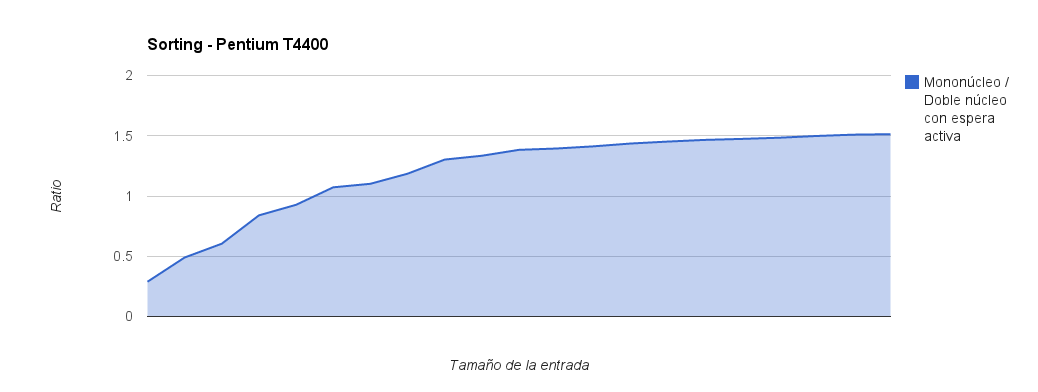
\includegraphics[height=6cm]{images/pentium_d_sorting.png}
\end{center}
En esta configuración podemos observar un cross-over en 64 elementos a partir de donde comienza a mejorar la performance utilizando dos cores. Para la mayor cantidad de elementos obtenemos una mejora aproximada del 50\%.
\subsubsection{Intel® Pentium® Processor T4200 - Vector modification}
\begin{center}
\begin{tabular}{|c|c|c|c|}
	\hline	
		Elements & MonoCore Ticks & DualCore Ticks & MonoCore Ticks/DualCore Ticks\\
	\hline	
		2 & 6528 & 103472 & 0.063\\
	\hline	
		4 & 8128 & 94672 & 0.085\\
	\hline	
		8 & 10656 & 106480 & 0.100\\
	\hline	
		16 & 14032 & 113328 & 0.123\\
	\hline	
		32 & 32688 & 77680 & 0.420\\
	\hline	
		64 & 60736 & 119088 & 0.510\\
	\hline	
		128 & 118432 & 187120 & 0.632\\
	\hline	
		256 & 237984 & 241904 & 0.983\\
	\hline	
		512 & 471664 & 382400 & 1.233\\
	\hline	
		1024 & 958848 & 801840 & 1.195\\
	\hline	
		2048 & 1862816 & 1618736 & 1.150\\
	\hline	
		4096 & 3616320 & 3241024 & 1.115\\
	\hline	
		8192 & 6855104 & 6129552 & 1.118\\
	\hline	
		16384 & 13412768 & 11785552 & 1.138\\
	\hline	
		32768 & 26840704 & 23272048 & 1.153\\
	\hline	
		65536 & 53739680 & 47434224 & 1.132\\
	\hline	
		131072 & 107571760 & 93427920 & 1.151\\
	\hline	
		262144 & 216317472 & 182467152 & 1.185\\
	\hline	
		524288 & 430617120 & 364908528 & 1.180\\
	\hline	
		1048576 & 860450928 & 745400768 & 1.154\\
	\hline	
		2097152 & 1730369088 & 1491881600 & 1.159\\
	\hline	
		4194304 & 3462956448 & 3000064512 & 1.154\\
	\hline
\end{tabular}
\end{center}
\begin{center}
    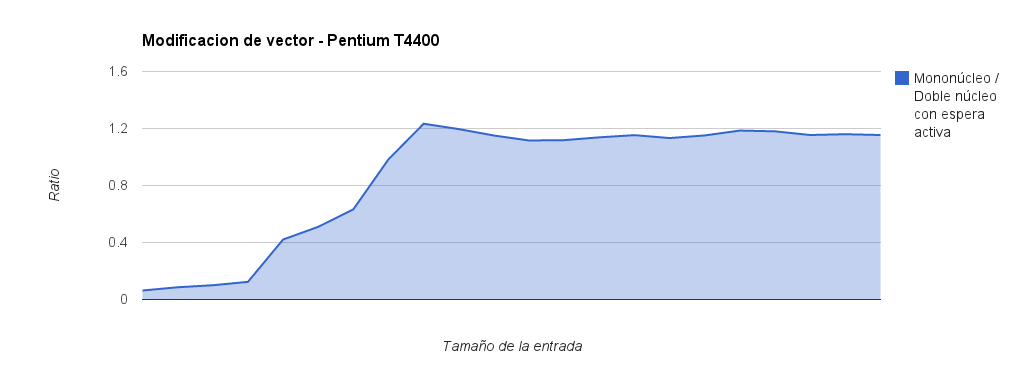
\includegraphics[height=6cm]{images/pentium_d_vectorsum.png}
\end{center}
Podemos observar como, incluso utilizando dos núcleos, la saturación del canal de memoria licua la performance mejorada del multiprocesamiento.

\subsubsection{Intel® Xeon® Processor E5345 - Sorting}
\begin{tabular}{|c|c|c|c|}
	\hline
		Elements & MonoCore Ticks & DualCore Ticks & MonoCore Ticks/DualCore Ticks\\
	\hline
		2 & 20657 & 34692 & 0.595\\
	\hline
		4 & 40565 & 47131 & 0.860\\
	\hline
		8 & 90559 & 73661 & 1.229\\
	\hline
		16 & 208635 & 137970 & 1.512\\
	\hline
		32 & 485933 & 287224 & 1.691\\
	\hline
		64 & 1096592 & 628369 & 1.745\\
	\hline
		128 & 2490712 & 1407854 & 1.769\\
	\hline
		256 & 5545589 & 3095624 & 1.791\\
	\hline
		512 & 12350142 & 6709311 & 1.840\\
	\hline
		1024 & 26958904 & 14815346 & 1.819\\
	\hline
		2048 & 58405928 & 32200161 & 1.813\\
	\hline
		4096 & 126362572 & 69358674 & 1.821\\
	\hline
		8192 & 271480069 & 149265949 & 1.818\\
	\hline
		16384 & 580168379 & 320822040 & 1.808\\
	\hline
		32768 & 1265098373 & 677863235 & 1.866\\
	\hline
		65536 & 2663953124 & 1447008150 & 1.841\\
	\hline
		131072 & 5597340728 & 3054159843 & 1.832\\
	\hline
		262144 & 11904206349 & 6435623397 & 1.849\\
	\hline
		524288 & 24800933899 & 13558975689 & 1.829\\
	\hline
		1048576 & 52289342196 & 28461202042 & 1.837\\
	\hline
		2097152 & 109516365196 & 59447473463 & 1.842\\
	\hline
\end{tabular}

	\begin{center}
	    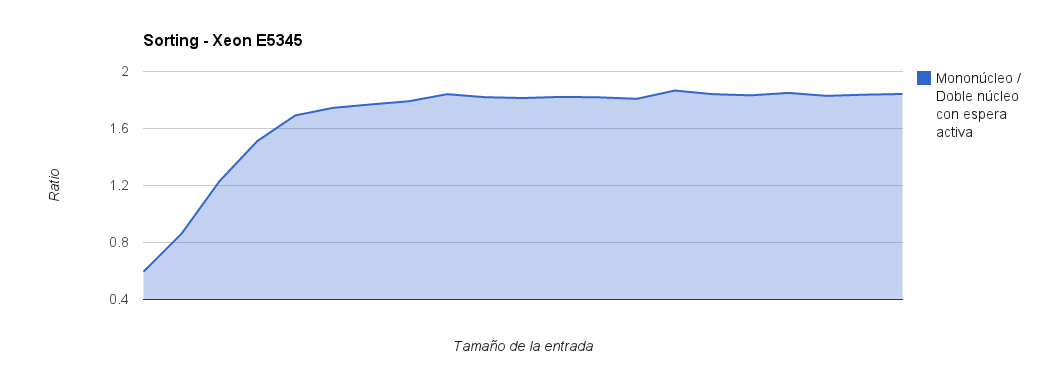
\includegraphics[height=6cm]{images/XEON_Sorting.png}
	\end{center}

	Dadas las mejores prestaciónes de caché y arquitectura de esta configuración, vemos que se obtiene un 84\% de mejora al realizar el multiprocesamiento al ordenar muestras de 2097152 elementos. El cross-over donde conviene utilizar multicore es muy bajo, desde 8 elementos ya es mas rápido el ordenamiento dual core. 

\subsubsection{Intel® Xeon® Processor E5345 - Vector modification}
\begin{center}
\begin{tabular}{|c|c|c|c|}
	\hline
		Elements & MonoCore Ticks & DualCore Ticks & MonoCore Ticks/DualCore Ticks\\
	\hline
		2 & 4900 & 16800 & 0.291\\
	\hline
		4 & 5831 & 17388 & 0.335\\
	\hline
		8 & 8211 & 17976 & 0.456\\
	\hline
		16 & 12985 & 19537 & 0.664\\
	\hline
		32 & 23198 & 26880 & 0.863\\
	\hline
		64 & 42511 & 35168 & 1.208\\
	\hline
		128 & 81543 & 55769 & 1.462\\
	\hline
		256 & 159663 & 94430 & 1.690\\
	\hline
		512 & 316463 & 210994 & 1.499\\
	\hline
		1024 & 630154 & 441224 & 1.428\\
	\hline
		2048 & 1256241 & 908292 & 1.383\\
	\hline
		4096 & 2509745 & 1836184 & 1.366\\
	\hline
		8192 & 5014814 & 3696385 & 1.356\\
	\hline
		16384 & 10030118 & 7422128 & 1.351\\
	\hline
		32768 & 20053355 & 14880299 & 1.347\\
	\hline
		65536 & 40102146 & 29786883 & 1.346\\
	\hline
		131072 & 80194310 & 59598644 & 1.345\\
	\hline
		262144 & 161790321 & 119193046 & 1.357\\
	\hline
		524288 & 327379871 & 238416367 & 1.373\\
	\hline
		1048576 & 656828004 & 478496431 & 1.372\\
	\hline
		2097152 & 1309034153 & 953788577 & 1.372\\
	\hline
		4194304 & 2619897161 & 1891070293 & 1.385\\
	\hline
\end{tabular}
\end{center}

	\begin{center}
	    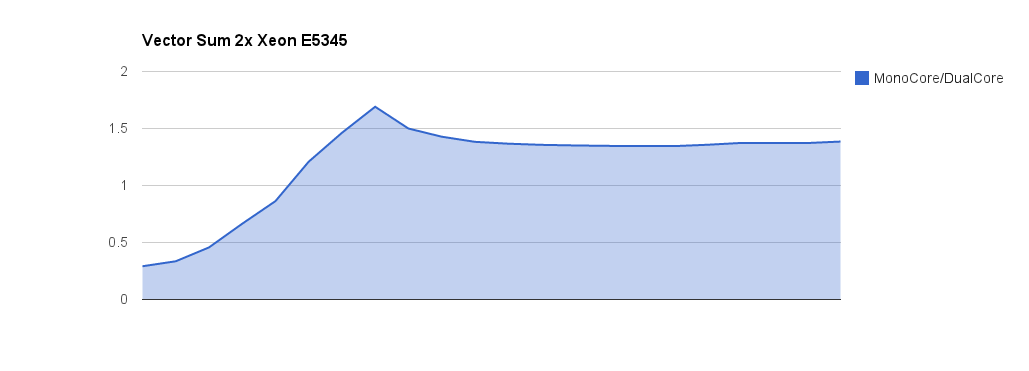
\includegraphics[height=6cm]{images/xeon_vector_sum.png}
	\end{center}

	Nuevamente los accesos a memoria afectan la performance del multiprocesamiento.

\subsubsection{Intel® Pentium® Processor G2030 - Sorting}
\begin{center}
	\begin{tabular}{|c|c|c|c|}
		\hline	
			Elements & MonoCore Ticks & DualCore Ticks & MonoCore Ticks/DualCore Ticks\\
		\hline
			2 & 15180 & 22996 & 0.660\\
		\hline
			4 & 30704 & 33812 & 0.908\\
		\hline
			8 & 70096 & 54804 & 1.279\\
		\hline
			16 & 186620 & 104288 & 1.789\\
		\hline
			32 & 436216 & 215084 & 2.028\\
		\hline
			64 & 1011620 & 473460 & 2.136\\
		\hline
			128 & 2311748 & 1074916 & 2.150\\
		\hline
			256 & 5156888 & 2393136 & 2.154\\
		\hline
			512 & 11414660 & 5290992 & 2.157\\
		\hline
			1024 & 25167592 & 11469944 & 2.194\\
		\hline
			2048 & 54610712 & 25100072 & 2.175\\
		\hline
			4096 & 118042804 & 57037548 & 2.069\\
		\hline
			8192 & 252518012 & 123304440 & 2.047\\
		\hline
			16384 & 536777312 & 264044108 & 2.032\\
		\hline
			32768 & 1097052680 & 555262936 & 1.975\\
		\hline
			65536 & 2322030308 & 1185902828 & 1.958\\
		\hline
			131072 & 4932183084 & 2539728536 & 1.942\\
		\hline
			262144 & 10447157964 & 5135427448 & 2.034\\
		\hline
			524288 & 21599239404 & 10835600988 & 1.993\\
		\hline
			1048576 & 45271465128 & 22793636612 & 1.986\\
		\hline
			2097152 & 94724393340 & 47526712420 & 1.993\\
		\hline
			4194304 & 197880816576 & 99686391488 & 1.985\\
		\hline
	\end{tabular}
\end{center}
	\begin{center}
	    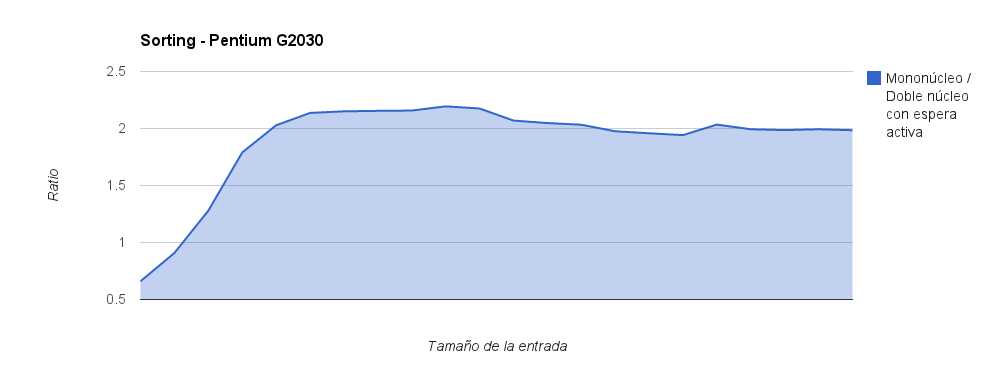
\includegraphics[height=6cm]{images/g2030_sorting.png}
	\end{center}

	Esta arquitectura nueva, nos sorprendió con un crossover de 8 elementos en el cual mejora la performance y a partir de 32 elementos aproximadamente se duplica el rendimiento utilizando multicore!
\subsubsection{Intel® Pentium® Processor G2030 - Vector modification}

\begin{center}
	\begin{tabular}{|c|c|c|c|}
		\hline	
			Elements & MonoCore Ticks & DualCore Ticks & MonoCore Ticks/DualCore Ticks\\
		\hline
			2 & 3844 & 7552 & 0.509\\
		\hline
			4 & 5260 & 7780 & 0.676\\
		\hline
			8 & 7996 & 10356 & 0.772\\
		\hline
			16 & 15036 & 12592 & 1.194\\
		\hline
			32 & 24732 & 18220 & 1.357\\
		\hline
			64 & 46612 & 32060 & 1.453\\
		\hline
			128 & 87408 & 55104 & 1.586\\
		\hline
			256 & 173268 & 128556 & 1.347\\
		\hline
			512 & 336340 & 198352 & 1.695\\
		\hline
			1024 & 682580 & 561132 & 1.216\\
		\hline
			2048 & 1356376 & 745136 & 1.820\\
		\hline
			4096 & 2959568 & 2184308 & 1.354\\
		\hline
			8192 & 6134040 & 4536436 & 1.352\\
		\hline
			16384 & 12473160 & 6453392 & 1.932\\
		\hline
			32768 & 24960936 & 18386228 & 1.357\\
		\hline
			65536 & 49965760 & 25624672 & 1.949\\
		\hline
			131072 & 99945548 & 74779612 & 1.336\\
		\hline
			262144 & 199857864 & 90879264 & 2.199\\
		\hline
			524288 & 399539592 & 285954068 & 1.397\\
		\hline
			1048576 & 799210112 & 381478298 & 2.095\\
		\hline
			2097152 & 1598536888 & 1196662984 & 1.335\\
		\hline
			4194304 & 3196868172 & 1601236716 & 1.996\\
		\hline
	\end{tabular}
\end{center}
	\begin{center}
	    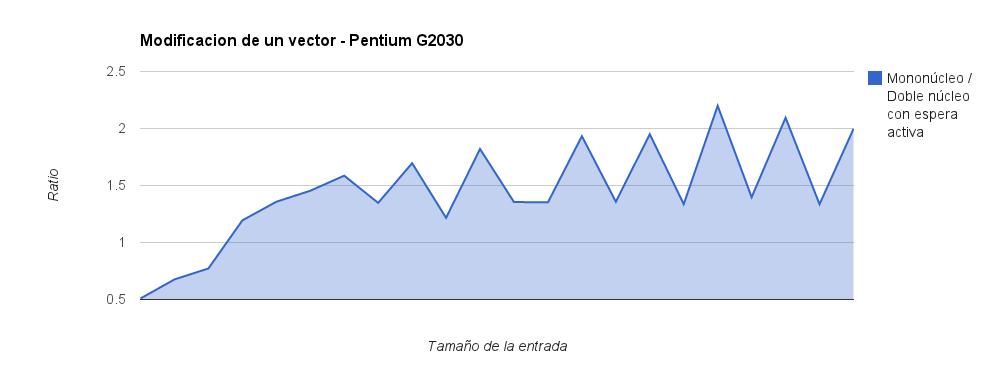
\includegraphics[height=6cm]{images/g2030_vectorsum.png}
	\end{center}

	A pesar de como afectan los accesos a memoria, en algunos casos vemos que se rompen los esquemas y se obtienen performances del doble versus procesamiento mono-núcleo.

\subsubsection{Intel® Core™ i7-920 Processor - Sorting - Vector modification }
\begin{center}
	\begin{tabular}{|c|c|c|c|c|c|c|}
		\hline	
			Elements & Sort Mono & Sort Dual & Vector Mono & Vector Dual & Sort Ratio & Vector Mod Ratio\\
		\hline
			2 & 17668 & 26204 & 4912 & 9332 & 0.674 & 0.526\\
		\hline
			4 & 36888 & 38648 & 5692 & 10680 & 0.954 & 0.532\\
		\hline
			8 & 84260 & 62436 & 8524 & 11696 & 1.349 & 0.728\\
		\hline
			16 & 192596 & 116900 & 15160 & 16356 & 1.647 & 0.926\\
		\hline
			32 & 463176 & 250716 & 26856 & 20256 & 1.847 & 1.325\\
		\hline
			64 & 1062000 & 549240 & 50600 & 32240 & 1.933 & 1.569\\
		\hline
			128 & 2427412 & 1236440 & 97260 & 55740 & 1.963 & 1.744\\
		\hline
			256 & 5389400 & 2719116 & 192860 & 122600 & 1.982 & 1.573\\
		\hline
			512 & 11997744 & 5903640 & 381276 & 260856 & 2.032 & 1.461\\
		\hline
			1024 & 25525608 & 13065240 & 761760 & 545620 & 1.953 & 1.396\\
		\hline
			2048 & 55905976 & 28463616 & 1519960 & 1110780 & 1.964 & 1.368\\
		\hline
			4096 & 120254264 & 69237000 & 3031636 & 2260796 & 1.736 & 1.340\\
		\hline
			8192 & 259149012 & 132442380 & 6051280 & 4509000 & 1.956 & 1.342\\
		\hline
			16384 & 554582312 & 284005796 & 12106900 & 9029180 & 1.952 & 1.340\\
		\hline
			32768 & 1199133428 & 612601980 & 24212436 & 12154760 & 1.957 & 1.992\\
		\hline
			65536 & 2547819264 & 1297609520 & 48417380 & 24300516 & 1.963 & 1.992\\
		\hline
			131072 & 5385534272 & 2769704056 & 96870560 & 48611840 & 1.944 & 1.992\\
		\hline
			262144 & 11395843660 & 5840527220 & 193900280 & 97191900 & 1.951 & 1.995\\
		\hline
			524288 & 23990990684 & 12323090580 & 398251576 & 299541500 & 1.946 & 1.329\\
		\hline
			1048576 & 50408173440 & 26217339456 & 792920300 & 395143060 & 1.922 & 2.006\\
		\hline
			2097152 & 105680965696 & 54178541700 & 1578620280 & 793110860 & 1.950 & 1.990\\
		\hline
			4194304 & 221064067796 & 113389632780 & 3176314036 & 2371198400 & 1.949 & 1.339\\
		\hline
	\end{tabular}
\end{center}

	\begin{center}
	    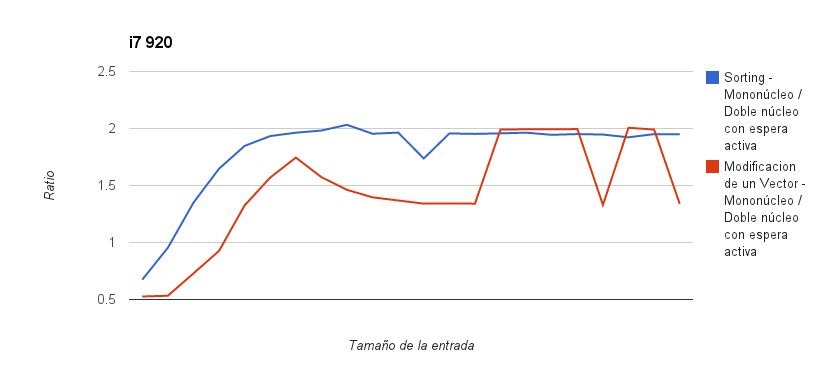
\includegraphics[height=7cm]{images/i7-vectorsum-sorting.png}
	\end{center}

	Podemos observar aqui que en arquitecturas mas nuevas de intel, se va mejorando la performance promedio obtenida, cada vez mas cercana a duplicar la performance single core, a pesar de esto, los accesos a memoria siguien siendo un problema en algunos casos.

\subsubsection{Intel® Core™ i5-2500K Processor - Sorting}
\begin{center}
	\begin{tabular}{|c|c|c|c|}
		\hline	
			Elements & MonoCore Ticks & DualCore Ticks & MonoCore Ticks/DualCore Ticks\\
		\hline
			2 & 15384 & 24580 & 0.625\\
		\hline
			4 & 31660 & 33112 & 0.956\\
		\hline
			8 & 74324 & 53544 & 1.388\\
		\hline
			16 & 171640 & 100236 & 1.712\\
		\hline
			32 & 406144 & 216452 & 1.876\\
		\hline
			64 & 932468 & 458840 & 2.032\\
		\hline
			128 & 2110364 & 1100608 & 1.917\\
		\hline
			256 & 4475012 & 2502924 & 1.787\\
		\hline
			512 & 9904452 & 5447160 & 1.818\\
		\hline
			1024 & 21732200 & 12102956 & 1.795\\
		\hline
			2048 & 47346996 & 26551652 & 1.783\\
		\hline
			4096 & 102885844 & 58287424 & 1.765\\
		\hline
			8192 & 222250916 & 120969120 & 1.837\\
		\hline
			16384 & 476876272 & 258581740 & 1.844\\
		\hline
			32768 & 1019406688 & 548013260 & 1.860\\
		\hline
			65536 & 2173616224 & 1186136300 & 1.832\\
		\hline
			131072 & 4633428528 & 2471420552 & 1.874\\
		\hline
			262144 & 9056811460 & 5190092924 & 1.745\\
		\hline
			524288 & 20854472344 & 10876582315 & 1.917\\
		\hline
			1048576 & 43923320368 & 23475758752 & 1.871\\
		\hline
			2097152 & 94551848940 & 49553049284 & 1.908\\
		\hline
			4194304 & 198157210936 & 103593610452 & 1.912\\
		\hline
	\end{tabular}
\end{center}
	\begin{center}
	    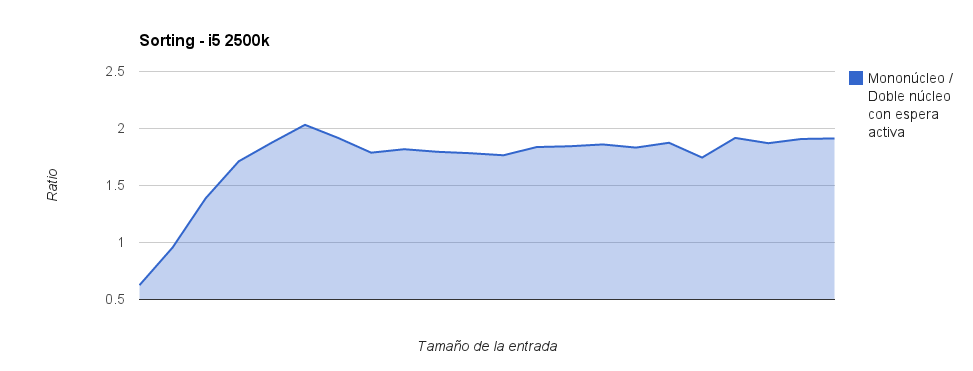
\includegraphics[height=6cm]{images/i5_sorting.png}
	\end{center}

	Dado que este procesador es cercano al i7, podemos observar una performance similar respecto a los ratios de mejora en multiprocesamiento, tanto en los ordenamientos, como en la modicación de vectores en al siguiente sección.

\subsubsection{Intel® Core™ i5-2500K Processor - Vector modification}
\begin{center}
	\begin{tabular}{|c|c|c|c|}
		\hline	
			Elements & MonoCore Ticks & DualCore Ticks & MonoCore Ticks/DualCore Ticks\\
		\hline
			2 & 3544 & 6900 & 0.513\\
		\hline
			4 & 5288 & 7280 & 0.726\\
		\hline
			8 & 7808 & 9868 & 0.791\\
		\hline
			16 & 13296 & 12132 & 1.095\\
		\hline
			32 & 23920 & 16980 & 1.408\\
		\hline
			64 & 47044 & 32276 & 1.457\\
		\hline
			128 & 92228 & 52192 & 1.767\\
		\hline
			256 & 182716 & 105168 & 1.737\\
		\hline
			512 & 363804 & 205808 & 1.767\\
		\hline
			1024 & 716228 & 394484 & 1.815\\
		\hline
			2048 & 1433180 & 786560 & 1.822\\
		\hline
			4096 & 2870572 & 1513800 & 1.896\\
		\hline
			8192 & 5694568 & 2914168 & 1.954\\
		\hline
			16384 & 11378960 & 5836656 & 1.949\\
		\hline
			32768 & 22432852 & 16351152 & 1.371\\
		\hline
			65536 & 45314096 & 22864312 & 1.981\\
		\hline
			131072 & 90536832 & 65673712 & 1.378\\
		\hline
			262144 & 181141232 & 91528392 & 1.979\\
		\hline
			524288 & 362184776 & 262148544 & 1.381\\
		\hline
			1048576 & 724287244 & 530532932 & 1.365\\
		\hline
			2097152 & 1448749484 & 1061714556 & 1.364\\
		\hline
			4194304 & 2897714296 & 1462866292 & 1.980\\
		\hline
	\end{tabular}
\end{center}
	\begin{center}
	    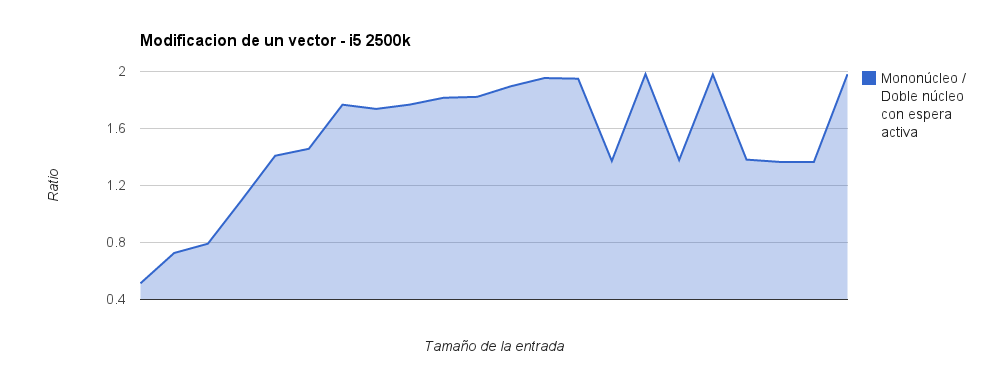
\includegraphics[height=6cm]{images/i5_vector_sum.png}
	\end{center}

\subsubsection{Intel® Core™2 Quad Processor Q6600 Sorting}
\begin{center}
\begin{tabular}{|c|c|c|c|}
	\hline	
		Elements & MonoCore Ticks & DualCore Ticks & MonoCore Ticks/DualCore Ticks\\
	\hline
		2 & 6885 & 16218 & 0.424\\
	\hline
		4 & 13277 & 18530 & 0.716\\
	\hline
		8 & 32011 & 30183 & 1.060\\
	\hline
		16 & 76364 & 56958 & 1.340\\
	\hline
		32 & 181024 & 120487 & 1.502\\
	\hline
		64 & 415990 & 252671 & 1.646\\
	\hline
		128 & 949399 & 560303 & 1.694\\
	\hline
		256 & 2121048 & 1218075 & 1.741\\
	\hline
		512 & 4742838 & 2604884 & 1.820\\
	\hline
		1024 & 10433809 & 5599078 & 1.863\\
	\hline
		2048 & 22765235 & 12013475 & 1.894\\
	\hline
		4096 & 49466056 & 25624066 & 1.930\\
	\hline
		8192 & 107050318 & 54191427 & 1.975\\
	\hline
		16384 & 230695245 & 119820352 & 1.925\\
	\hline
		32768 & 492634993 & 242634115 & 2.030\\
	\hline
		65536 & 1054223219 & 535990263 & 1.966\\
	\hline
		131072 & 2249860461 & 1087838729 & 2.068\\
	\hline
		262144 & 4773926137 & 2274182829 & 2.099\\
	\hline
		524288 & 10087422167 & 4892424806 & 2.061\\
	\hline
		1048576 & 21270642148 & 10335385475 & 2.058\\
	\hline
		2097152 & 44667373988 & 21181628542 & 2.108\\
	\hline
		4194304 & 93526794057 & 44040620699 & 2.123\\
	\hline
\end{tabular}
\end{center}

	\begin{center}
	    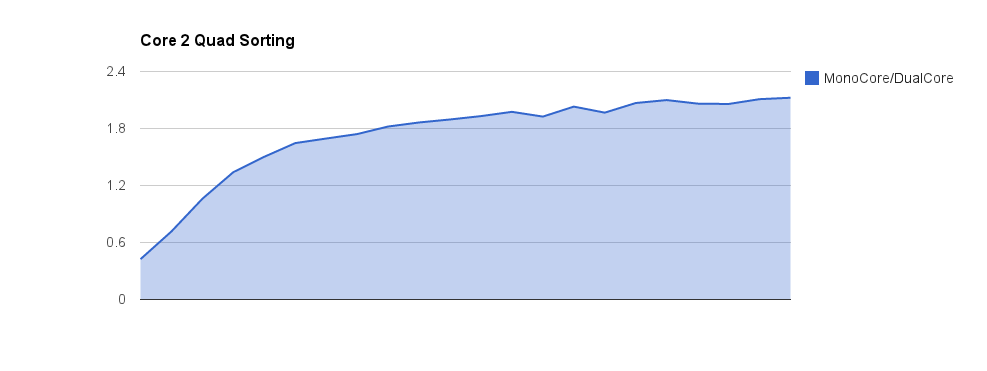
\includegraphics[height=6cm]{images/core2quad_sorting.png}
	\end{center}

	Esta arquitectura, a pesar de ser mas antigua de los ix, nos muestra una buena performance utilizando multicore, de aproximadamente el doble, la mejora respecto de la cantidad de elementos en aumento es casi instantanea, a partir de 8 elementos.

\subsubsection{Intel® Core™2 Quad Processor Q6600 Vector modification}
\begin{center}
	\begin{tabular}{|c|c|c|c|}
		\hline	
			Elements & MonoCore Ticks & DualCore Ticks & MonoCore Ticks/DualCore Ticks\\
		\hline
				2 & 1717 & 5695 & 0.301\\
		\hline
				4 & 1938 & 6945 & 0.279\\
		\hline
				8 & 2456 & 6945 & 0.353\\
		\hline
				16 & 5491 & 9826 & 0.558\\
		\hline
				32 & 13745 & 13515 & 1.017\\
		\hline
				64 & 28016 & 18309 & 1.530\\
		\hline
				128 & 56151 & 32266 & 1.740\\
		\hline
				256 & 115379 & 68434 & 1.685\\
		\hline
				512 & 231107 & 150314 & 1.537\\
		\hline
				1024 & 459255 & 307930 & 1.491\\
		\hline
				2048 & 918060 & 623645 & 1.472\\
		\hline
				4096 & 1835176 & 1292867 & 1.419\\
		\hline
				8192 & 3682583 & 2606517 & 1.412\\
		\hline
				16384 & 7390283 & 5332679 & 1.385\\
		\hline
				32768 & 14743522 & 10669702 & 1.381\\
		\hline
				65536 & 29898164 & 20515192 & 1.457\\
		\hline
				131072 & 59790649 & 40836465 & 1.464\\
		\hline
				262144 & 119581808 & 83774122 & 1.427\\
		\hline
				524288 & 239160938 & 167648356 & 1.426\\
		\hline
				1048576 & 478114256 & 332301831 & 1.438\\
		\hline
				2097152 & 957119720 & 661399399 & 1.447\\
		\hline
				4194304 & 1913099785 & 1352226444 & 1.414\\
		\hline
	\end{tabular}
\end{center}
	\begin{center}
	    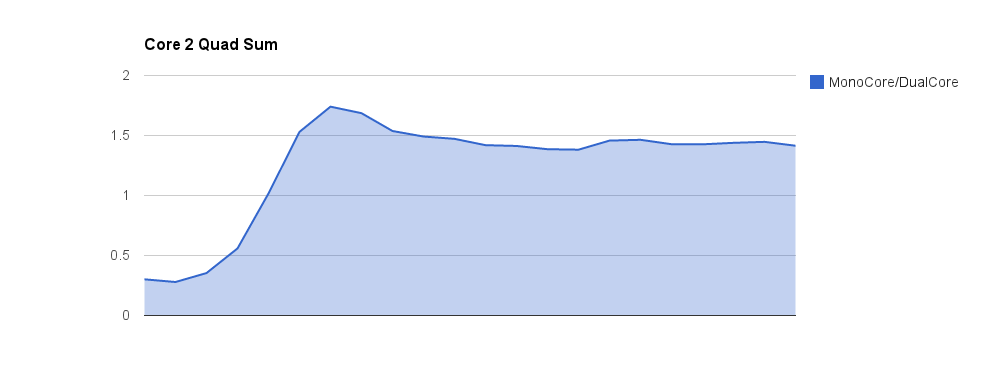
\includegraphics[height=6cm]{images/core2quad_sum.png}
	\end{center}

	Los accesos a memoria, a los cuales compiten los 2 cores, afectan el rendimiento, aunque utilizar dos cores sigue dando aproximadamente un 40\% de mejoría.
	
\subsubsection{Intel® Pentium® Processor T4200 - Sorting usando Inter-processor interrupts}

Para intentar reducir los accesos a memoria, implementamos la sincronización entre núcleos mediante interrupciones entre procesadores en lugar de realizar espera activa a memoria. Los resultados fueron curiosos, dado que dió peor la performance respecto a la sincronización con variables en memoria RAM. Creemos que esto se debe a las velocidades del bus de memoria y el bus de sistema y la memoria caché.

\begin{center}
	\begin{tabular}{|c|c|c|c|c|c|c|}
		\hline	
			Elements & Sort Single & Sort Dual Mem & Sort Dual Ipi & Ratio M/I & Single/DMem & Single/DIpi\\
		\hline
			2 & 26336 & 55088 & 123712 & 0.445  & 0.478  & 0.212 \\
		\hline
			4 & 51136 & 70896 & 164496 & 0.430  & 0.721  & 0.310 \\
		\hline
			8 & 114832 & 108224 & 272560 & 0.397  & 1.061 & 0.421 \\
		\hline
			16 & 268832 & 213984 & 363696 & 0.588  & 1.256 & 0.739 \\
		\hline
			32 & 613520 & 455376 & 571488 & 0.796  & 1.347 & 1.073 \\
		\hline
			64 & 1429152 & 951840 & 1063760 & 0.894  & 1.501 & 1.343 \\
		\hline
			128 & 2524576 & 2182176 & 2280608 & 0.956  & 1.156 & 1.106 \\
		\hline
			256 & 7816560 & 4642912 & 4782544 & 0.970  & 1.683 & 1.634 \\
		\hline
			512 & 17833216 & 9749392 & 10258304 & 0.950  & 1.829 & 1.738 \\
		\hline
			1024 & 37187824 & 20810160 & 22367904 & 0.930 & 1.787 & 1.662 \\
		\hline
			2048 & 79244560 & 44773584 & 49540224 & 0.903  & 1.769 & 1.599 \\
		\hline
			4096 & 171885520 & 95302656 & 107242560 & 0.888  & 1.803 & 1.602 \\
		\hline
			8192 & 369363168 & 191632704 & 221836560 & 0.863  & 1.927 & 1.665 \\
		\hline
			16384 & 781349776 & 401270912 & 473079168 & 0.848  & 1.947 & 1.651 \\
		\hline
			32768 & 1670361776 & 882252640 & 1065852080 & 0.827  & 1.893 & 1.567 \\
		\hline
			65536 & 3568050464 & 1873549072 & 2277199056 & 0.822  & 1.904 & 1.566 \\
		\hline
			131072 & 7538692864 & 3718695296 & 4572378768 & 0.813  & 2.027 & 1.648 \\
		\hline
			262144 & 15870953952 & 7744017984 & 9611314224 & 0.805  & 2.049 & 1.651 \\
		\hline
			524288 & 33266571168 & 16705027472 & 21105461872 & 0.791  & 1.991 & 1.576 \\
		\hline
			1048576 & 69926858336 & 34701409440 & 44269003616 & 0.783  & 2.015 & 1.579 \\
		\hline
			2097152 & 146290056320 & 72153753040 & 92620047520 & 0.779  & 2.027 & 1.579 \\
		\hline
			4194304 & 305621530000 & 149990136352 & 193768043584 & 0.774  & 2.037 & 1.577 \\
		\hline
	\end{tabular}
\end{center}

	\begin{center}
	    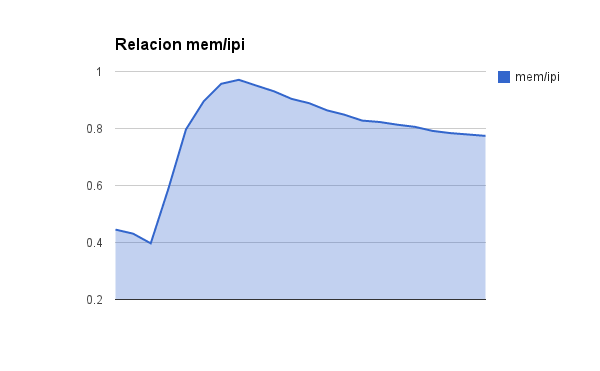
\includegraphics[height=7cm]{images/pentium_d_mem_ipi.png}
	\end{center}

	\begin{center}
	    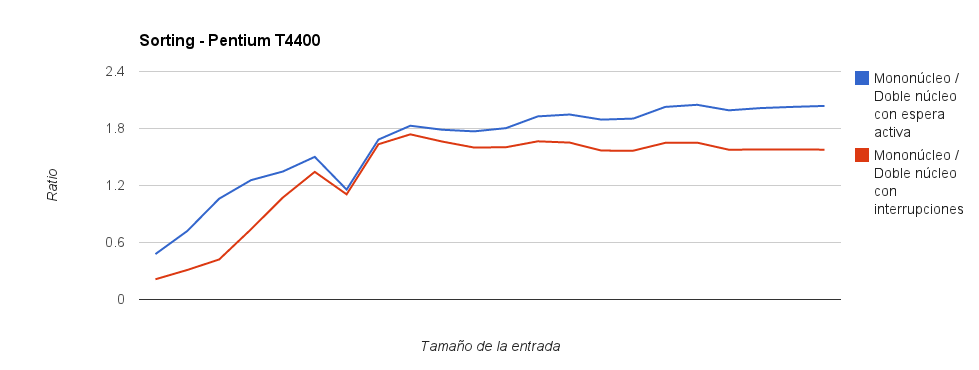
\includegraphics[height=6cm]{images/pentium_d_gain_mono_mem_mono_ipi.png}
	\end{center}

\subsubsection{Intel® Pentium® Processor G2030 - Sorting usando Inter-processor interrupts}

\begin{center}
	\begin{tabular}{|c|c|c|c|c|c|c|}
		\hline	
			Elements & Sort Single & Sort Dual Mem & Sort Dual Ipi & Ratio M/I & Single/DMem & Single/DIpi\\
		\hline
			2 & 15452 & 21896 & 102700 & 0.213 & 0.705 & 0.150\\
		\hline
			4 & 29912 & 32196 & 110408 & 0.291 & 0.929 & 0.270\\
		\hline
			8 & 71836 & 50516 & 134456 & 0.375 & 1.422 & 0.534\\
		\hline
			16 & 169000 & 103400 & 183016 & 0.564 & 1.634 & 0.923\\
		\hline
			32 & 397952 & 211700 & 310164 & 0.682 & 1.879 & 1.283\\
		\hline
			64 & 916460 & 471424 & 565800 & 0.833 & 1.944 & 1.619\\
		\hline
			128 & 2139260 & 1090936 & 1181260 & 0.923 & 1.960 & 1.810\\
		\hline
			256 & 4788876 & 2416744 & 2549880 & 0.947 & 1.981 & 1.878\\
		\hline
			512 & 10815520 & 5308704 & 5487300 & 0.967 & 2.037 & 1.971\\
		\hline
			1024 & 23706116 & 11522124 & 11979292 & 0.961 & 2.057 & 1.978\\
		\hline
			2048 & 51881936 & 25373340 & 25050724 & 1.012 & 2.044 & 2.071\\
		\hline
			4096 & 112622828 & 56403280 & 57929704 & 0.973 & 1.996 & 1.944\\
		\hline
			8192 & 241852140 & 121972712 & 124943688 & 0.976 & 1.982 & 1.935\\
		\hline
			16384 & 515303872 & 262110928 & 266906044 & 0.982 & 1.965 & 1.930\\
		\hline
			32768 & 1138315716 & 556395036 & 564395308 & 0.985 & 2.045 & 2.016\\
		\hline
			65536 & 2328303276 & 1185656408 & 1198435060 & 0.989 & 1.963 & 1.942\\
		\hline
			131072 & 5102082740 & 2520384000 & 2552306004 & 0.987 & 2.024 & 1.999\\
		\hline
			262144 & 10786122552 & 5146255024 & 5192631012 & 0.991 & 2.095 & 2.077\\
		\hline
			524288 & 21983866092 & 10830150400 & 10945820376 & 0.989 & 2.029 & 2.008\\
		\hline
			1048576 & 46087236500 & 22837077648 & 23007268768 & 0.992 & 2.018 & 2.003\\
		\hline
			2097152 & 97382977980 & 47855259656 & 48355560760 & 0.989 & 2.034 & 2.013\\
		\hline
			4194304 & 203101063672 & 100389365112 & 100937254332 & 0.994 & 2.023 & 2.012\\
		\hline
	\end{tabular}
\end{center}

\begin{center}
	    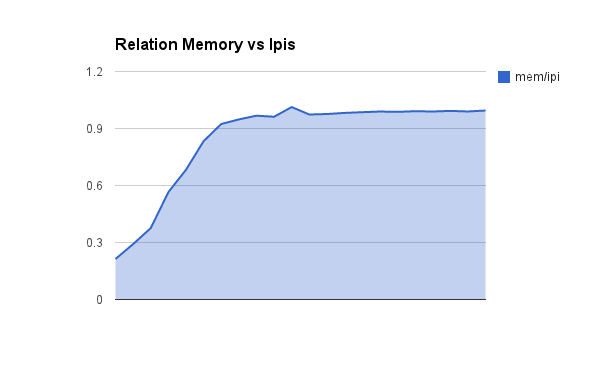
\includegraphics[height=7cm]{images/memory_ipis_g2030_sortipi.png}
	\end{center}


\begin{center}
	    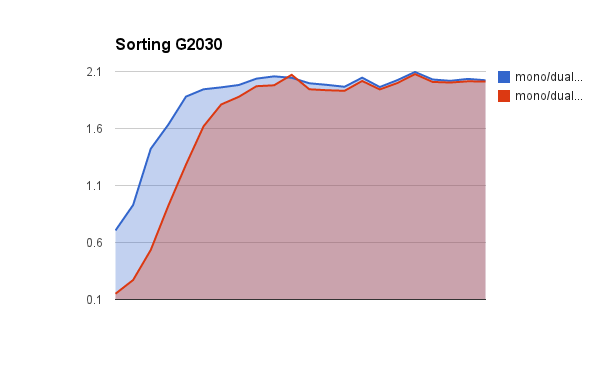
\includegraphics[height=6cm]{images/sort_ipis_g2030.png}
	\end{center}


Dada la velocidad superior del bus de sistema y las nuevas tecnologías de caché de la arquitectura se ve una mejoria respecto al procesador Pentium D T4200 al momento de comparar sincronización entre memoria e ipis. 

\subsubsection{Intel® Pentium® Processor T4200 - FFT Single - FFT Dual Mem - FFT Dual IPI}

\begin{center}
	\begin{tabular}{|c|c|c|c|c|c|}
		\hline	
			Elements & FFT Single & FFT Dual Mem & FFT Dual Ipi & Single/DMem & Single/DIpi\\
		\hline
			2 & 70832 & 92672 & 94400 & 0.764 & 0.750\\
		\hline
			4 & 178464 & 229536 & 284256 & 0.777 & 0.627\\
		\hline
			8 & 420560 & 517824 & 671888 & 0.812 & 0.625\\
		\hline
			16 & 1247232 & 1132416 & 1502656 & 1.101 & 0.830\\
		\hline
			32 & 2860176 & 2475856 & 3286000 & 1.155 & 0.870\\
		\hline
			64 & 6449744 & 5451264 & 7063456 & 1.183 & 0.913\\
		\hline
			128 & 14460480 & 11873856 & 15290304 & 1.217 & 0.945\\
		\hline
			256 & 32076304 & 25889856 & 32869536 & 1.238 & 0.975\\
		\hline
			512 & 70559488 & 56002208 & 70211568 & 1.259 & 1.004\\
		\hline
			1024 & 154010400 & 120728848 & 149749936 & 1.275 & 1.028\\
		\hline
			2048 & 323222368 & 257452224 & 317900272 & 1.255 & 1.016\\
		\hline
			4096 & 701196608 & 552926256 & 675095392 & 1.268 & 1.038\\
		\hline
			8192 & 1521703040 & 1185646304 & 1429235616 & 1.283 & 1.064\\
		\hline
			16384 & 3270511200 & 2522381008 & 3018106480 & 1.296 & 1.083\\
		\hline
	\end{tabular}
\end{center}


\begin{center}
	    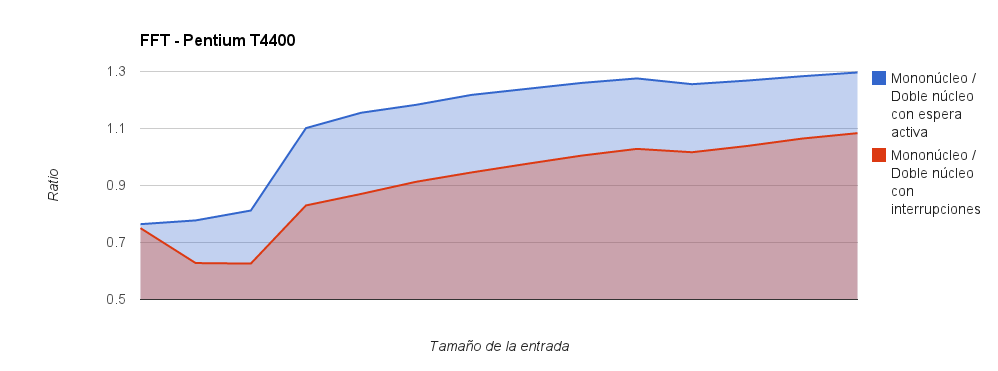
\includegraphics[height=6cm]{images/fft_pentiumd.png}
	\end{center}

	Se obtiene una mejora utilizando dual core a partir de los 16 elementos, culminando en un 30\% de mejora en la máxima cantidad testeada. En esta arquitectura el uso de IPIS no es muy favorable respecto a la sincronización por memoria.


\subsubsection{Intel® Core™2 Quad Processor Q6600 - FFT Single - FFT Dual Mem - FFT Dual IPI}

\begin{center}
	\begin{tabular}{|c|c|c|c|c|c|}
		\hline	
			Elements & FFT Single & FFT Dual Mem & FFT Dual Ipi & Single/DMem & Single/DIpi\\
		\hline
			2 & 28815 & 29427 & 29385 & 0.979 & 0.980\\
		\hline
			4 & 72845 & 70329 & 101031 & 1.035 & 0.721\\
		\hline
			8 & 173103 & 155848 & 194199 & 1.110 & 0.891\\
		\hline
			16 & 404991 & 344539 & 433483 & 1.175 & 0.934\\
		\hline
			32 & 924281 & 750856 & 949297 & 1.230 & 0.973\\
		\hline
			64 & 2098420 & 1639624 & 2054917 & 1.279 & 1.021\\
		\hline
			128 & 4705387 & 3568818 & 4415665 & 1.318 & 1.065\\
		\hline
			256 & 10448327 & 7752374 & 9476531 & 1.347 & 1.102\\
		\hline
			512 & 23017286 & 16735140 & 20251377 & 1.375 & 1.136\\
		\hline
			1024 & 50295528 & 36675672 & 43080728 & 1.371 & 1.167\\
		\hline
			2048 & 109147616 & 77031496 & 91376640 & 1.416 & 1.194\\
		\hline
			4096 & 235491488 & 165446541 & 193718867 & 1.423 & 1.215\\
		\hline
			8192 & 505322288 & 350143806 & 408601570 & 1.443 & 1.236\\
		\hline
			16384 & 1080310024 & 740571382 & 860584064 & 1.458 & 1.255\\
		\hline
	\end{tabular}
\end{center}

\begin{center}
	    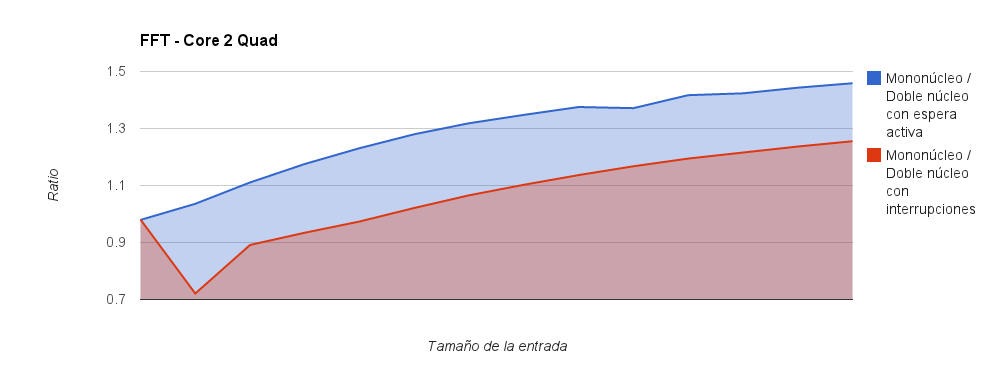
\includegraphics[height=6cm]{images/fft_core2quad.png}
	\end{center}

Vemos como en esta arquitectura mejora contra la anterior la mejora máxima, de un 46\%. Las ipis todavia no son demasiado favorables, además se observa que el cross-over para la mejora en dual core es casi instantaneo sobre la cantidad de elementos.

\subsubsection{Intel® Core™ i5-2500K Processor - FFT Single - FFT Dual Mem - FFT Dual IPI}

\begin{center}
	\begin{tabular}{|c|c|c|c|c|c|}
		\hline	
			Elements & FFT Single & FFT Dual Mem & FFT Dual Ipi & Single/DMem & Single/DIpi\\
		\hline
			2 & 77784 & 82284 & 78968 & 0.945 & 0.985\\
		\hline
			4 & 214688 & 191236 & 216976 & 1.122 & 0.989\\
		\hline
			8 & 514696 & 428148 & 502068 & 1.202 & 1.025\\
		\hline
			16 & 1215252 & 927192 & 1114204 & 1.310 & 1.090\\
		\hline
			32 & 2802900 & 2014076 & 2419752 & 1.391 & 1.158\\
		\hline
			64 & 6360344 & 4367528 & 5236460 & 1.456 & 1.214\\
		\hline
			128 & 14268528 & 9535292 & 11246792 & 1.496 & 1.268\\
		\hline
			256 & 31695828 & 20575104 & 24102060 & 1.540 & 1.315\\
		\hline
			512 & 69969592 & 44330152 & 51512984 & 1.578 & 1.358\\
		\hline
			1024 & 153126636 & 95175168 & 109542068 & 1.608 & 1.397\\
		\hline
			2048 & 332522532 & 203051852 & 231857552 & 1.637 & 1.434\\
		\hline
			4096 & 717823008 & 432009528 & 489417964 & 1.661 & 1.466\\
		\hline
			8192 & 1541572072 & 916023644 & 1030637576 & 1.682 & 1.495\\
		\hline
			16384 & 3296190392 & 1937514232 & 2166612988 & 1.701 & 1.521\\
		\hline
	\end{tabular}
\end{center}

\begin{center}
	    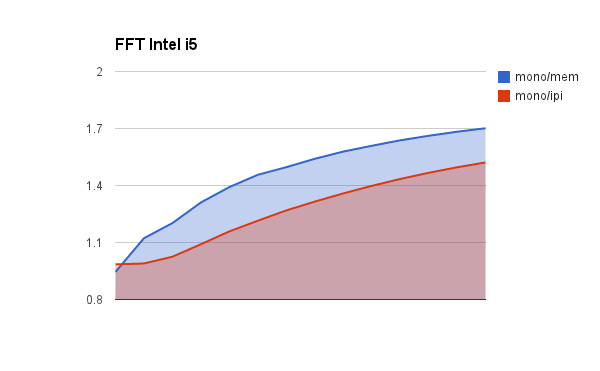
\includegraphics[height=6cm]{images/fft_i5.png}
	\end{center}
En la arquitectura del core i5, mejora el rendimiento obtenido utilizando multicore, otorgando un 70\% de mejora versus monoprocesamiento. Las ipis proveen un 52\% de mejora, además observamos que el cross-over para la mejora en dual core es casi instantaneo sobre la cantidad de elementos.

\subsubsection{Intel® Pentium® Processor G2030 - FFT Single - FFT Dual Mem - FFT Dual IPI}

\begin{center}
	\begin{tabular}{|c|c|c|c|c|c|}
		\hline	
			Elements & FFT Single & FFT Dual Mem & FFT Dual Ipi & Single/DMem & Single/DIpi\\
		\hline
			2 & 75888 & 80812 & 77972 & 0.939 & 0.973\\
		\hline
			4 & 209524 & 191800 & 220424 & 1.092 & 0.950\\
		\hline
			8 & 514828 & 426920 & 510424 & 1.205 & 1.008\\
		\hline
			16 & 1205000 & 938892 & 1142776 & 1.283 & 1.054\\
		\hline
			32 & 2760068 & 2047208 & 2490212 & 1.348 & 1.108\\
		\hline
			64 & 6291332 & 4508696 & 5387504 & 1.395 & 1.167\\
		\hline
			128 & 14026052 & 9758488 & 11629396 & 1.437 & 1.206\\
		\hline
			256 & 31301112 & 21347084 & 24994892 & 1.466 & 1.252\\
		\hline
			512 & 69070356 & 46043584 & 53512760 & 1.500 & 1.290\\
		\hline
			1024 & 150448296 & 98699668 & 113700712 & 1.524 & 1.323\\
		\hline
			2048 & 325692216 & 211210216 & 241297652 & 1.542 & 1.349\\
		\hline
			4096 & 702220892 & 450242892 & 511164280 & 1.559 & 1.373\\
		\hline
			8192 & 1507872220 & 957204752 & 1079792760 & 1.575 & 1.396\\
		\hline
			16384 & 3222351048 & 2028073172 & 2273867600 & 1.588 & 1.417\\
		\hline
	\end{tabular}
\end{center}


\begin{center}
	    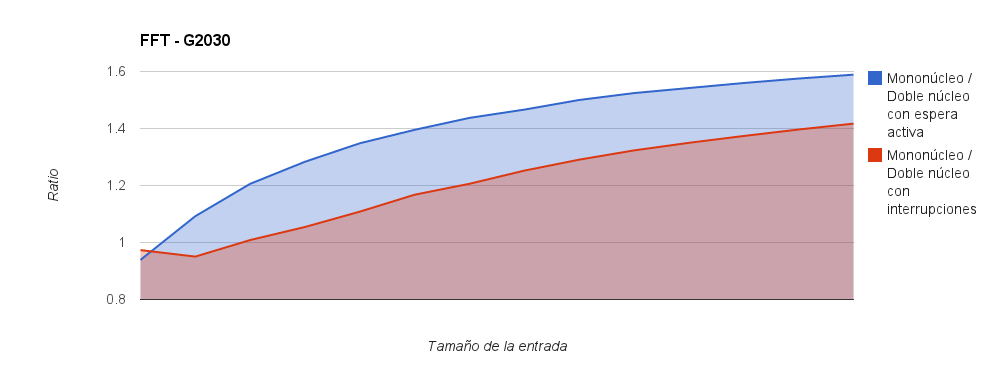
\includegraphics[height=6cm]{images/fft_g2030.png}
	\end{center}

Aqui obtenemos una mejora maxima de un 59\%, el cross-over es casi instantaneo y mejoran bastante las ipis, en relación a su contraparte sincronizada por espera activa con accesos a memoria al compararse con monoprocesamiento.

\subsubsection{Intel® Xeon® Processor E5345 - FFT Single - FFT Dual Mem - FFT Dual IPI}

\begin{center}
	\begin{tabular}{|c|c|c|c|c|c|}
		\hline	
			Elements & FFT Single & FFT Dual Mem & FFT Dual Ipi & Single/DMem & Single/DIpi\\
		\hline
			2 & 93429 & 97160 & 97314 & 0.961 & 0.960\\
		\hline
			4 & 245973 & 231707 & 271544 & 1.061 & 0.905\\
		\hline
			8 & 597730 & 509642 & 627865 & 1.172 & 0.952\\
		\hline
			16 & 1394330 & 1109801 & 1382430 & 1.256 & 1.008\\
		\hline
			32 & 3210844 & 2413852 & 2992248 & 1.330 & 1.073\\
		\hline
			64 & 7297927 & 5258589 & 6447819 & 1.387 & 1.131\\
		\hline
			128 & 16403002 & 11400445 & 13845454 & 1.438 & 1.184\\
		\hline
			256 & 36485239 & 24669883 & 29654149 & 1.478 & 1.230\\
		\hline
			512 & 80414341 & 53201029 & 63250026 & 1.511 & 1.271\\
		\hline
			1024 & 175866670 & 114169888 & 134506631 & 1.540 & 1.307\\
		\hline
			2048 & 383665926 & 244086430 & 284939466 & 1.571 & 1.346\\
		\hline
			4096 & 831156431 & 512455125 & 590454613 & 1.621 & 1.407\\
		\hline
			8192 & 1799559559 & 1083358444 & 1262194136 & 1.661 & 1.425\\
		\hline
			16384 & 3789572983 & 2328605440 & 2658443333 & 1.627 & 1.425\\
		\hline
	\end{tabular}
\end{center}

\begin{center}
	    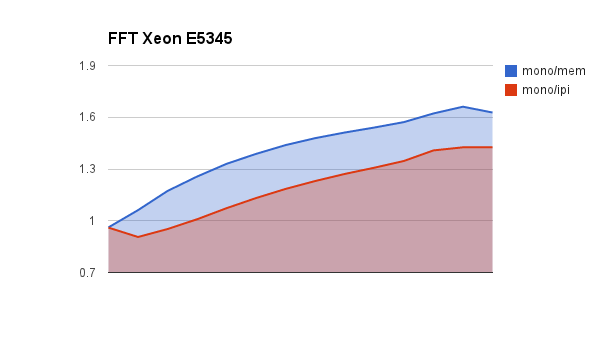
\includegraphics[height=5cm]{images/fft_xeon_e5345.png}
\end{center}

En esta máquina se obtuvo un valor máximo de un 63\% de mejora entre single y dual core con espera activa, el cross-over es a partir de 4 elementos y la arquitectura brinda una mejora de 42\% respecto a las ipis contra single core.

\subsubsection{Intel® Pentium® Processor G2030 - FFT Single - FFT Dual Mem - FFT Dual IPI - Corregido parámetro cross-over}

\begin{center}
	\begin{tabular}{|c|c|c|c|c|c|}
		\hline	
			Elements & FFT Single & FFT Dual Mem & FFT Dual Ipi & Single/DMem & Single/DIpi\\
		\hline
			2 & 76928 & 80184 & 77008 & 0.959 & 0.998\\
		\hline
			4 & 209344 & 209876 & 209620 & 0.997 & 0.998\\
		\hline
			8 & 509544 & 504388 & 508344 & 1.010 & 1.002\\
		\hline
			16 & 1204652 & 1095428 & 1136104 & 1.099 & 1.060\\
		\hline
			32 & 2769940 & 2375436 & 2468452 & 1.166 & 1.122\\
		\hline
			64 & 6285460 & 5116232 & 5351456 & 1.228 & 1.174\\
		\hline
			128 & 14118780 & 11058380 & 11609068 & 1.276 & 1.216\\
		\hline
			256 & 31421656 & 23805852 & 24912928 & 1.319 & 1.261\\
		\hline
			512 & 69159148 & 50957916 & 53272104 & 1.357 & 1.298\\
		\hline
			1024 & 150365428 & 108450908 & 113057384 & 1.386 & 1.329\\
		\hline
			2048 & 325566300 & 230628592 & 239963220 & 1.411 & 1.356\\
		\hline
			4096 & 701862512 & 488929320 & 508322008 & 1.435 & 1.380\\
		\hline
			8192 & 1507207556 & 1034818916 & 1075238928 & 1.456 & 1.401\\
		\hline
			16384 & 3220958472 & 2182392616 & 2262842272 & 1.475 & 1.423\\
		\hline
	\end{tabular}
\end{center}

\begin{center}
	    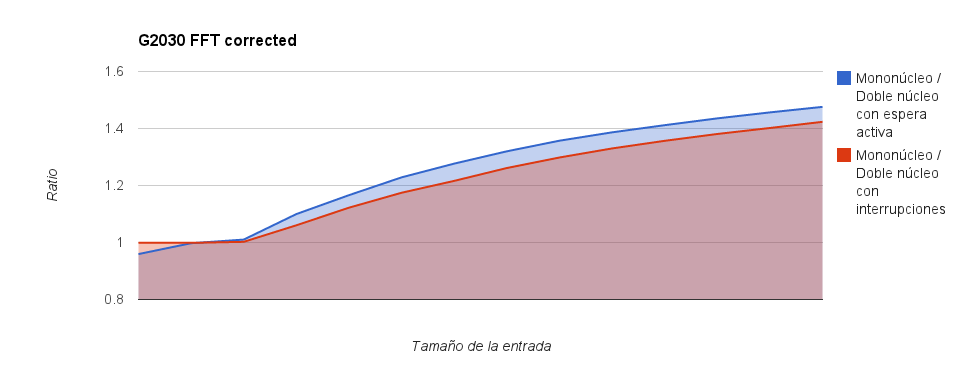
\includegraphics[height=6cm]{images/fft_g2030_corrected.png}
\end{center}

\subsubsection{Intel® Pentium® Processor T4200 - FFT Single - FFT Dual Mem - FFT Dual IPI - Corregido parámetro cross-over}

\begin{center}
	\begin{tabular}{|c|c|c|c|c|c|}
		\hline	
			Elements & FFT Single & FFT Dual Mem & FFT Dual Ipi & Single/DMem & Single/DIpi\\
		\hline
			2 & 35761 & 35805 & 35486 & 0.998 & 1.007\\
		\hline
			4 & 90915 & 91388 & 92862 & 0.994 & 0.979\\
		\hline
			8 & 217316 & 214940 & 219373 & 1.011 & 0.990\\
		\hline
			16 & 509124 & 465883 & 501732 & 1.092 & 1.014\\
		\hline
			32 & 1173953 & 1007820 & 1092289 & 1.164 & 1.074\\
		\hline
			64 & 2669315 & 2171323 & 2385240 & 1.229 & 1.119\\
		\hline
			128 & 5989203 & 4716437 & 5155986 & 1.269 & 1.161\\
		\hline
			256 & 13300727 & 10159050 & 11098527 & 1.309 & 1.198\\
		\hline
			512 & 29302328 & 21799811 & 23799919 & 1.344 & 1.231\\
		\hline
			1024 & 64078740 & 46520694 & 50830560 & 1.377 & 1.260\\
		\hline
			2048 & 139116241 & 99224873 & 108137887 & 1.402 & 1.286\\
		\hline
			4096 & 302052850 & 212169727 & 230777096 & 1.423 & 1.308\\
		\hline
			8192 & 648160260 & 447351124 & 486158453 & 1.448 & 1.333\\
		\hline
			16384 & 1385888295 & 944842954 & 1026775189 & 1.466 & 1.349\\
		\hline
	\end{tabular}
\end{center}

\begin{center}
    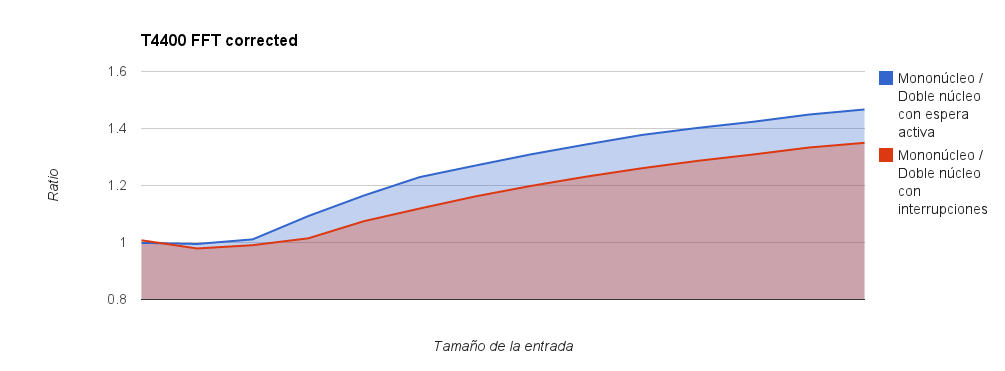
\includegraphics[height=6cm]{images/fft_pentiumd_corrected.png}
\end{center}
